\documentclass{standalone}
\usepackage{tikz}
\usetikzlibrary{patterns, positioning}

\begin{document}
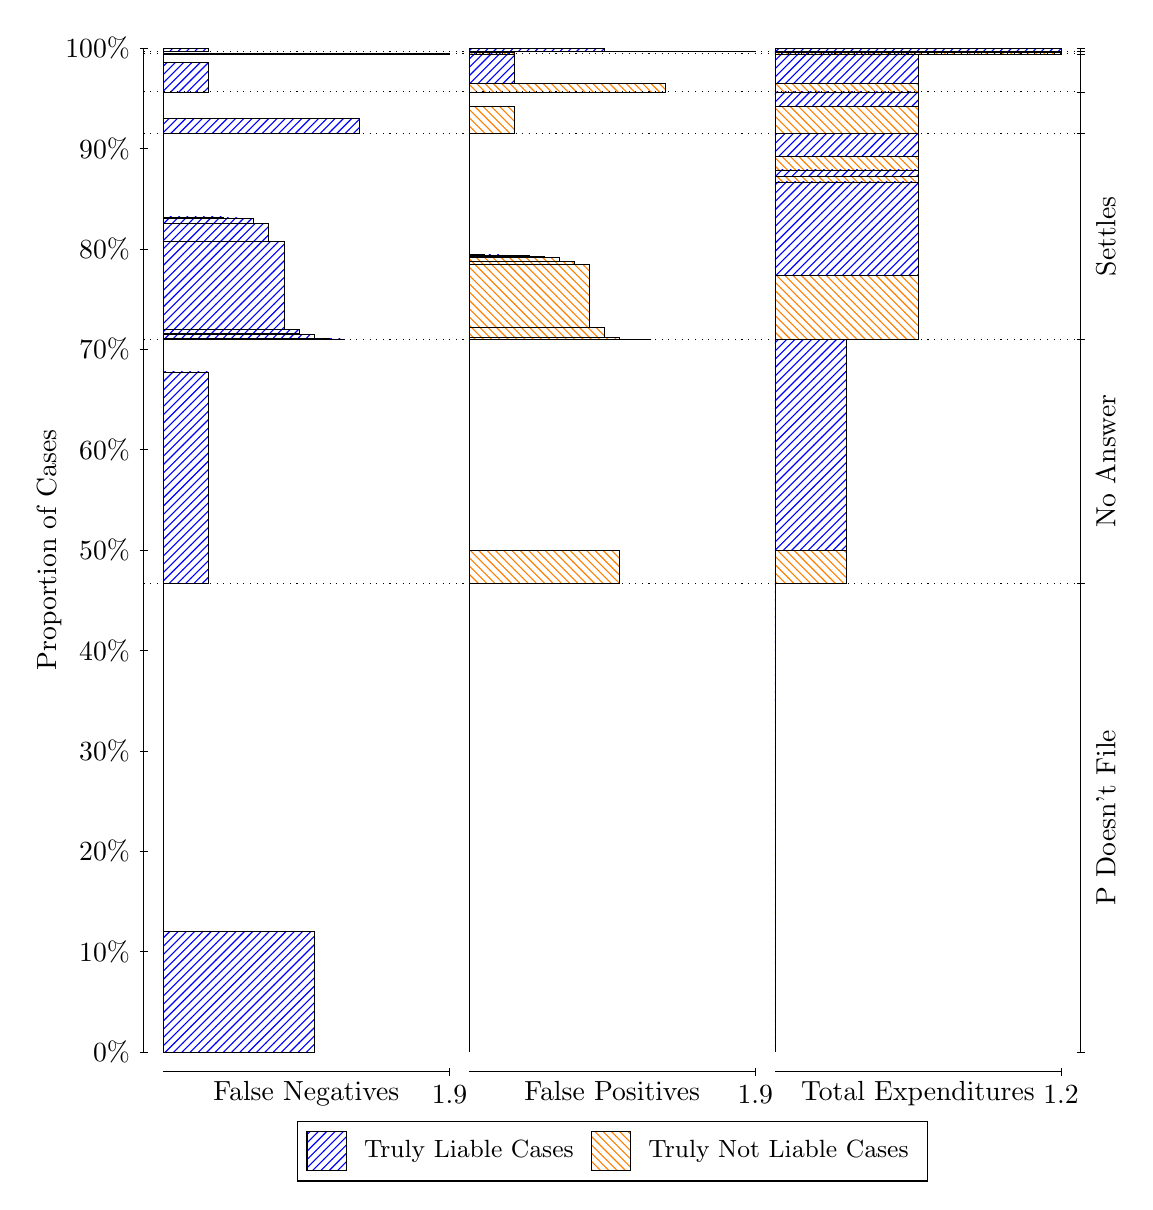
\begin{tikzpicture}
\draw[black, very thin] (1.5,1.75) -- (1.5,14.5);
\node[rotate=90, anchor=center] at (0.3, 8.125) {Proportion of Cases};
\draw[black, very thin] (1.45,1.75) -- (1.55,1.75);
\node[anchor=east] at (1.45, 1.75) {0\%};
\draw[black, very thin] (1.45,3.025) -- (1.55,3.025);
\node[anchor=east] at (1.45, 3.025) {10\%};
\draw[black, very thin] (1.45,4.3) -- (1.55,4.3);
\node[anchor=east] at (1.45, 4.3) {20\%};
\draw[black, very thin] (1.45,5.575) -- (1.55,5.575);
\node[anchor=east] at (1.45, 5.575) {30\%};
\draw[black, very thin] (1.45,6.85) -- (1.55,6.85);
\node[anchor=east] at (1.45, 6.85) {40\%};
\draw[black, very thin] (1.45,8.125) -- (1.55,8.125);
\node[anchor=east] at (1.45, 8.125) {50\%};
\draw[black, very thin] (1.45,9.4) -- (1.55,9.4);
\node[anchor=east] at (1.45, 9.4) {60\%};
\draw[black, very thin] (1.45,10.675) -- (1.55,10.675);
\node[anchor=east] at (1.45, 10.675) {70\%};
\draw[black, very thin] (1.45,11.95) -- (1.55,11.95);
\node[anchor=east] at (1.45, 11.95) {80\%};
\draw[black, very thin] (1.45,13.225) -- (1.55,13.225);
\node[anchor=east] at (1.45, 13.225) {90\%};
\draw[black, very thin] (1.45,14.5) -- (1.55,14.5);
\node[anchor=east] at (1.45, 14.5) {100\%};

\draw[black, very thin] (13.4,1.75) -- (13.4,14.5);
\draw[black, very thin] (13.35,1.75) -- (13.45,1.75);
\node[anchor=west] at (13.35, 1.75) {};
\draw[black, very thin] (13.35,7.7032) -- (13.45,7.7032);
\node[anchor=west] at (13.35, 7.7032) {};
\draw[black, very thin] (13.35,10.8) -- (13.45,10.8);
\node[anchor=west] at (13.35, 10.8) {};
\draw[black, very thin] (13.35,13.417) -- (13.45,13.417);
\node[anchor=west] at (13.35, 13.417) {};
\draw[black, very thin] (13.35,13.944) -- (13.45,13.944);
\node[anchor=west] at (13.35, 13.944) {};
\draw[black, very thin] (13.35,14.426) -- (13.45,14.426);
\node[anchor=west] at (13.35, 14.426) {};
\draw[black, very thin] (13.35,14.455) -- (13.45,14.455);
\node[anchor=west] at (13.35, 14.455) {};
\draw[black, very thin] (13.35,14.5) -- (13.45,14.5);
\node[anchor=west] at (13.35, 14.5) {};

\draw[black, very thin, pattern color=blue, pattern=north east lines] (1.75,1.75) rectangle (3.6623,3.285);
\draw[black, very thin, pattern color=orange, pattern=north west lines] (1.75,3.285) rectangle (1.75,7.7032);
\draw[black, very thin, pattern color=blue, pattern=north east lines] (1.75,7.7032) rectangle (2.3237,10.386);
\draw[black, very thin, pattern color=orange, pattern=north west lines] (1.75,10.386) rectangle (1.75,10.8);
\draw[black, very thin, pattern color=blue, pattern=north east lines] (1.75,10.8) rectangle (4.0447,10.805);
\draw[black, very thin, pattern color=blue, pattern=north east lines] (1.75,10.805) rectangle (3.8535,10.809);
\draw[black, very thin, pattern color=blue, pattern=north east lines] (1.75,10.809) rectangle (3.6623,10.866);
\draw[black, very thin, pattern color=blue, pattern=north east lines] (1.75,10.866) rectangle (3.4711,10.878);
\draw[black, very thin, pattern color=blue, pattern=north east lines] (1.75,10.878) rectangle (3.4711,10.931);
\draw[black, very thin, pattern color=blue, pattern=north east lines] (1.75,10.931) rectangle (3.2798,12.041);
\draw[black, very thin, pattern color=blue, pattern=north east lines] (1.75,12.041) rectangle (3.0886,12.271);
\draw[black, very thin, pattern color=blue, pattern=north east lines] (1.75,12.271) rectangle (2.8974,12.339);
\draw[black, very thin, pattern color=blue, pattern=north east lines] (1.75,12.339) rectangle (2.7061,12.344);
\draw[black, very thin, pattern color=blue, pattern=north east lines] (1.75,12.344) rectangle (2.5149,12.355);
\draw[black, very thin, pattern color=orange, pattern=north west lines] (1.75,12.355) rectangle (1.75,13.417);
\draw[black, very thin, pattern color=blue, pattern=north east lines] (1.75,13.417) rectangle (4.236,13.603);
\draw[black, very thin, pattern color=orange, pattern=north west lines] (1.75,13.603) rectangle (1.75,13.944);
\draw[black, very thin, pattern color=blue, pattern=north east lines] (1.75,13.944) rectangle (2.3237,14.315);
\draw[black, very thin, pattern color=orange, pattern=north west lines] (1.75,14.315) rectangle (1.75,14.426);
\draw[black, very thin, pattern color=blue, pattern=north east lines] (1.75,14.426) rectangle (5.3833,14.433);
\draw[black, very thin, pattern color=orange, pattern=north west lines] (1.75,14.433) rectangle (1.75,14.455);
\draw[black, very thin, pattern color=blue, pattern=north east lines] (1.75,14.455) rectangle (2.3237,14.493);
\draw[black, very thin, pattern color=orange, pattern=north west lines] (1.75,14.493) rectangle (1.75,14.5);
\draw[black, very thin, pattern color=orange, pattern=north west lines] (5.6333,1.75) rectangle (5.6333,6.1682);
\draw[black, very thin, pattern color=blue, pattern=north east lines] (5.6333,6.1682) rectangle (5.6333,7.7032);
\draw[black, very thin, pattern color=orange, pattern=north west lines] (5.6333,7.7032) rectangle (7.5456,8.1175);
\draw[black, very thin, pattern color=blue, pattern=north east lines] (5.6333,8.1175) rectangle (5.6333,10.8);
\draw[black, very thin, pattern color=orange, pattern=north west lines] (5.6333,10.8) rectangle (7.9281,10.802);
\draw[black, very thin, pattern color=orange, pattern=north west lines] (5.6333,10.802) rectangle (7.7368,10.803);
\draw[black, very thin, pattern color=orange, pattern=north west lines] (5.6333,10.803) rectangle (7.5456,10.827);
\draw[black, very thin, pattern color=orange, pattern=north west lines] (5.6333,10.827) rectangle (7.3544,10.956);
\draw[black, very thin, pattern color=orange, pattern=north west lines] (5.6333,10.956) rectangle (7.1632,11.748);
\draw[black, very thin, pattern color=orange, pattern=north west lines] (5.6333,11.748) rectangle (6.9719,11.795);
\draw[black, very thin, pattern color=orange, pattern=north west lines] (5.6333,11.795) rectangle (6.7807,11.843);
\draw[black, very thin, pattern color=orange, pattern=north west lines] (5.6333,11.843) rectangle (6.5895,11.85);
\draw[black, very thin, pattern color=orange, pattern=north west lines] (5.6333,11.85) rectangle (6.3982,11.862);
\draw[black, very thin, pattern color=blue, pattern=north east lines] (5.6333,11.862) rectangle (6.0158,11.873);
\draw[black, very thin, pattern color=blue, pattern=north east lines] (5.6333,11.873) rectangle (5.8246,11.879);
\draw[black, very thin, pattern color=blue, pattern=north east lines] (5.6333,11.879) rectangle (5.6333,13.417);
\draw[black, very thin, pattern color=orange, pattern=north west lines] (5.6333,13.417) rectangle (6.207,13.758);
\draw[black, very thin, pattern color=blue, pattern=north east lines] (5.6333,13.758) rectangle (5.6333,13.944);
\draw[black, very thin, pattern color=orange, pattern=north west lines] (5.6333,13.944) rectangle (8.1193,14.055);
\draw[black, very thin, pattern color=blue, pattern=north east lines] (5.6333,14.055) rectangle (6.207,14.426);
\draw[black, very thin, pattern color=orange, pattern=north west lines] (5.6333,14.426) rectangle (6.207,14.448);
\draw[black, very thin, pattern color=blue, pattern=north east lines] (5.6333,14.448) rectangle (5.6333,14.455);
\draw[black, very thin, pattern color=orange, pattern=north west lines] (5.6333,14.455) rectangle (9.2667,14.462);
\draw[black, very thin, pattern color=blue, pattern=north east lines] (5.6333,14.462) rectangle (7.3544,14.5);
\draw[black, very thin, pattern color=orange, pattern=north west lines] (9.5167,1.75) rectangle (9.5167,6.1682);
\draw[black, very thin, pattern color=blue, pattern=north east lines] (9.5167,6.1682) rectangle (9.5167,7.7032);
\draw[black, very thin, pattern color=orange, pattern=north west lines] (9.5167,7.7032) rectangle (10.425,8.1175);
\draw[black, very thin, pattern color=blue, pattern=north east lines] (9.5167,8.1175) rectangle (10.425,10.8);
\draw[black, very thin, pattern color=orange, pattern=north west lines] (9.5167,10.8) rectangle (11.333,11.616);
\draw[black, very thin, pattern color=blue, pattern=north east lines] (9.5167,11.616) rectangle (11.333,12.799);
\draw[black, very thin, pattern color=orange, pattern=north west lines] (9.5167,12.799) rectangle (11.333,12.873);
\draw[black, very thin, pattern color=blue, pattern=north east lines] (9.5167,12.873) rectangle (11.333,12.951);
\draw[black, very thin, pattern color=orange, pattern=north west lines] (9.5167,12.951) rectangle (11.333,13.122);
\draw[black, very thin, pattern color=blue, pattern=north east lines] (9.5167,13.122) rectangle (11.333,13.417);
\draw[black, very thin, pattern color=orange, pattern=north west lines] (9.5167,13.417) rectangle (11.333,13.758);
\draw[black, very thin, pattern color=blue, pattern=north east lines] (9.5167,13.758) rectangle (11.333,13.944);
\draw[black, very thin, pattern color=orange, pattern=north west lines] (9.5167,13.944) rectangle (11.333,14.055);
\draw[black, very thin, pattern color=blue, pattern=north east lines] (9.5167,14.055) rectangle (11.333,14.426);
\draw[black, very thin, pattern color=orange, pattern=north west lines] (9.5167,14.426) rectangle (13.15,14.448);
\draw[black, very thin, pattern color=blue, pattern=north east lines] (9.5167,14.448) rectangle (13.15,14.455);
\draw[black, very thin, pattern color=orange, pattern=north west lines] (9.5167,14.455) rectangle (13.15,14.462);
\draw[black, very thin, pattern color=blue, pattern=north east lines] (9.5167,14.462) rectangle (13.15,14.5);
\draw[black, dotted] (1.5,7.7032) -- (13.4,7.7032);
\draw[black, dotted] (1.5,10.8) -- (13.4,10.8);
\draw[black, dotted] (1.5,13.417) -- (13.4,13.417);
\draw[black, dotted] (1.5,13.944) -- (13.4,13.944);
\draw[black, dotted] (1.5,14.426) -- (13.4,14.426);
\draw[black, dotted] (1.5,14.455) -- (13.4,14.455);
\draw[black, very thin] (1.75,1.5) -- (5.3833,1.5);
\node[anchor=north] at (3.5667, 1.5) {False Negatives};
\draw[black, very thin] (5.3833,1.45) -- (5.3833,1.55);
\node[anchor=north] at (5.3833, 1.45) {1.9};

\draw[black, very thin] (5.6333,1.5) -- (9.2667,1.5);
\node[anchor=north] at (7.45, 1.5) {False Positives};
\draw[black, very thin] (9.2667,1.45) -- (9.2667,1.55);
\node[anchor=north] at (9.2667, 1.45) {1.9};

\draw[black, very thin] (9.5167,1.5) -- (13.15,1.5);
\node[anchor=north] at (11.333, 1.5) {Total Expenditures};
\draw[black, very thin] (13.15,1.45) -- (13.15,1.55);
\node[anchor=north] at (13.15, 1.45) {1.2};

\node[black, centered, rotate=90] at (13.72, 4.7266) {P Doesn't File};
\node[black, centered, rotate=90] at (13.72, 9.2517) {No Answer};
\node[black, centered, rotate=90] at (13.72, 12.109) {Settles};





\draw (7.449999999999999,1.5) node[draw=none] (baseCoordinate) {};
\begin{scope}[align=center]
        \matrix[scale=0.5, draw=black, below=0.5cm of baseCoordinate, nodes={draw}, column sep=0.1cm]{
            \node[rectangle, draw, minimum width=0.5cm, minimum height=0.5cm, pattern=north east lines, pattern color=blue] {}; &
            \node[draw=none, font=\small] (B) {Truly Liable Cases}; &
            \node[rectangle, draw, minimum width=0.5cm, minimum height=0.5cm, pattern=north west lines, pattern color=orange] {}; &
            \node[draw=none, font=\small] (B) {Truly Not Liable Cases}; \\
            };
\end{scope}

\end{tikzpicture}
\end{document}